\section{Revised Solution Design}
\label{sec:revised_solution_design}

The Basilisk platform is missing some key functionality to run benchmarking jobs successfully.
In this section, we describe the designed solutions for the shortcomings listed in section \ref{sec:architecture_review}.


\subsection{Code Refactoring}
\label{sec:impl_code_refactor}
As stated in section \ref{sec:code_refactor}, an in-depth code refactoring was recommended.
Before designing and implementing new functionality, we performed an in-depth refactoring and restructuring of the code base.
This resulted in a clean code base on which all future implementations can be built.


\subsection{Management of Repositories and Configurations}
\label{sec:management_repo_config_design}
In section \ref{sec:management_repo_config} we explained the problem of storing and managing repositories, the corresponding hooks and the \ts{}-configurations between the \acf{hcs} and the \acf{jms}.

Different solutions were considered for merging the functionality of the two services.

In the designed solution, the management and storing of the repositories are moved into the \ac{jms}.
This includes the corresponding REST endpoints and internal logic of the \ac{hcs} that are needed for the management.
The different repositories (\gh{} and \dockh{}) are added over the REST API of the \ac{jms}.

In section \ref{sec:review_missing_impl} (\acl{hcs}) it is listed, that the \ac{hcs} is missing the REST endpoints for deleting repositories.
Since the repository management is moved to the \ac{jms}, these endpoints are also added there.
\\

The \ac{jms} communicates with the \ac{hcs} over RabbitMQ message queues.
Through these messages, the \ac{hcs} gets the needed information about the repositories it should observe.
These include the URL and for \gh{} repositories details like the observed branch and potentially an OAuth token for authenticating with the API.

The functionality used when a new release is found does not need to be changed.
When a new release is found, the \ac{hcs} still sends a message containing the relevant information about the release to the \ac{jms}.
\\

Figure \ref{fig:repo_management_restructure} shows the restructured REST APIs and the adjusted messaging between \ac{hcs} and \ac{jms}.

\begin{figure}[tbph]
	\centering
	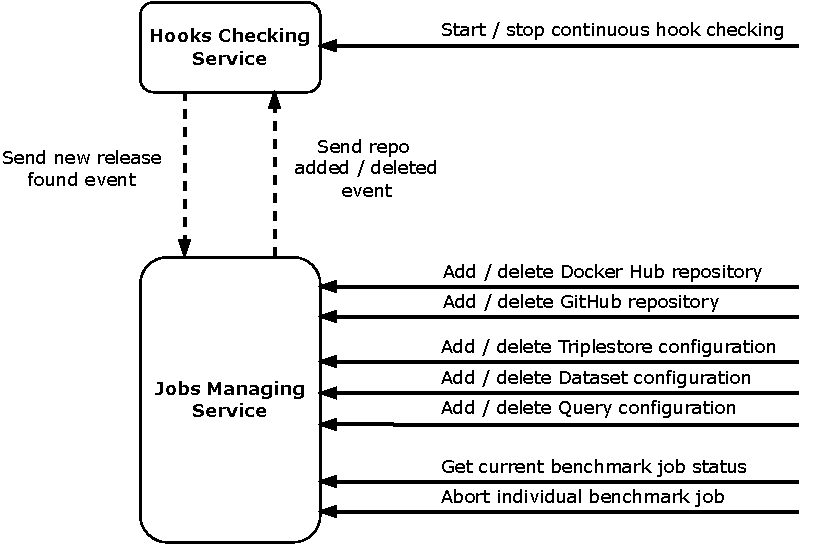
\includegraphics[width=.65\textwidth]{figures/messaging-implementation-hcs-jms.pdf}
	\caption{Overview of the restructured REST APIs and adjusted messaging}
	\label{fig:repo_management_restructure}
\end{figure}



\subsection{Restructure of Data Models in the \acl{jms}}
\label{sec:data_model_restructure_jms}
In section \ref{sec:review_data_model}, we reviewed the data model used for storing and managing the different configuration types inside the \ac{jms}.
To mitigate the stated problems with the data model, we designed the database schema shown in figure \ref{fig:design_jms_db_schema}.

\begin{figure}[tbph]
	\centering
	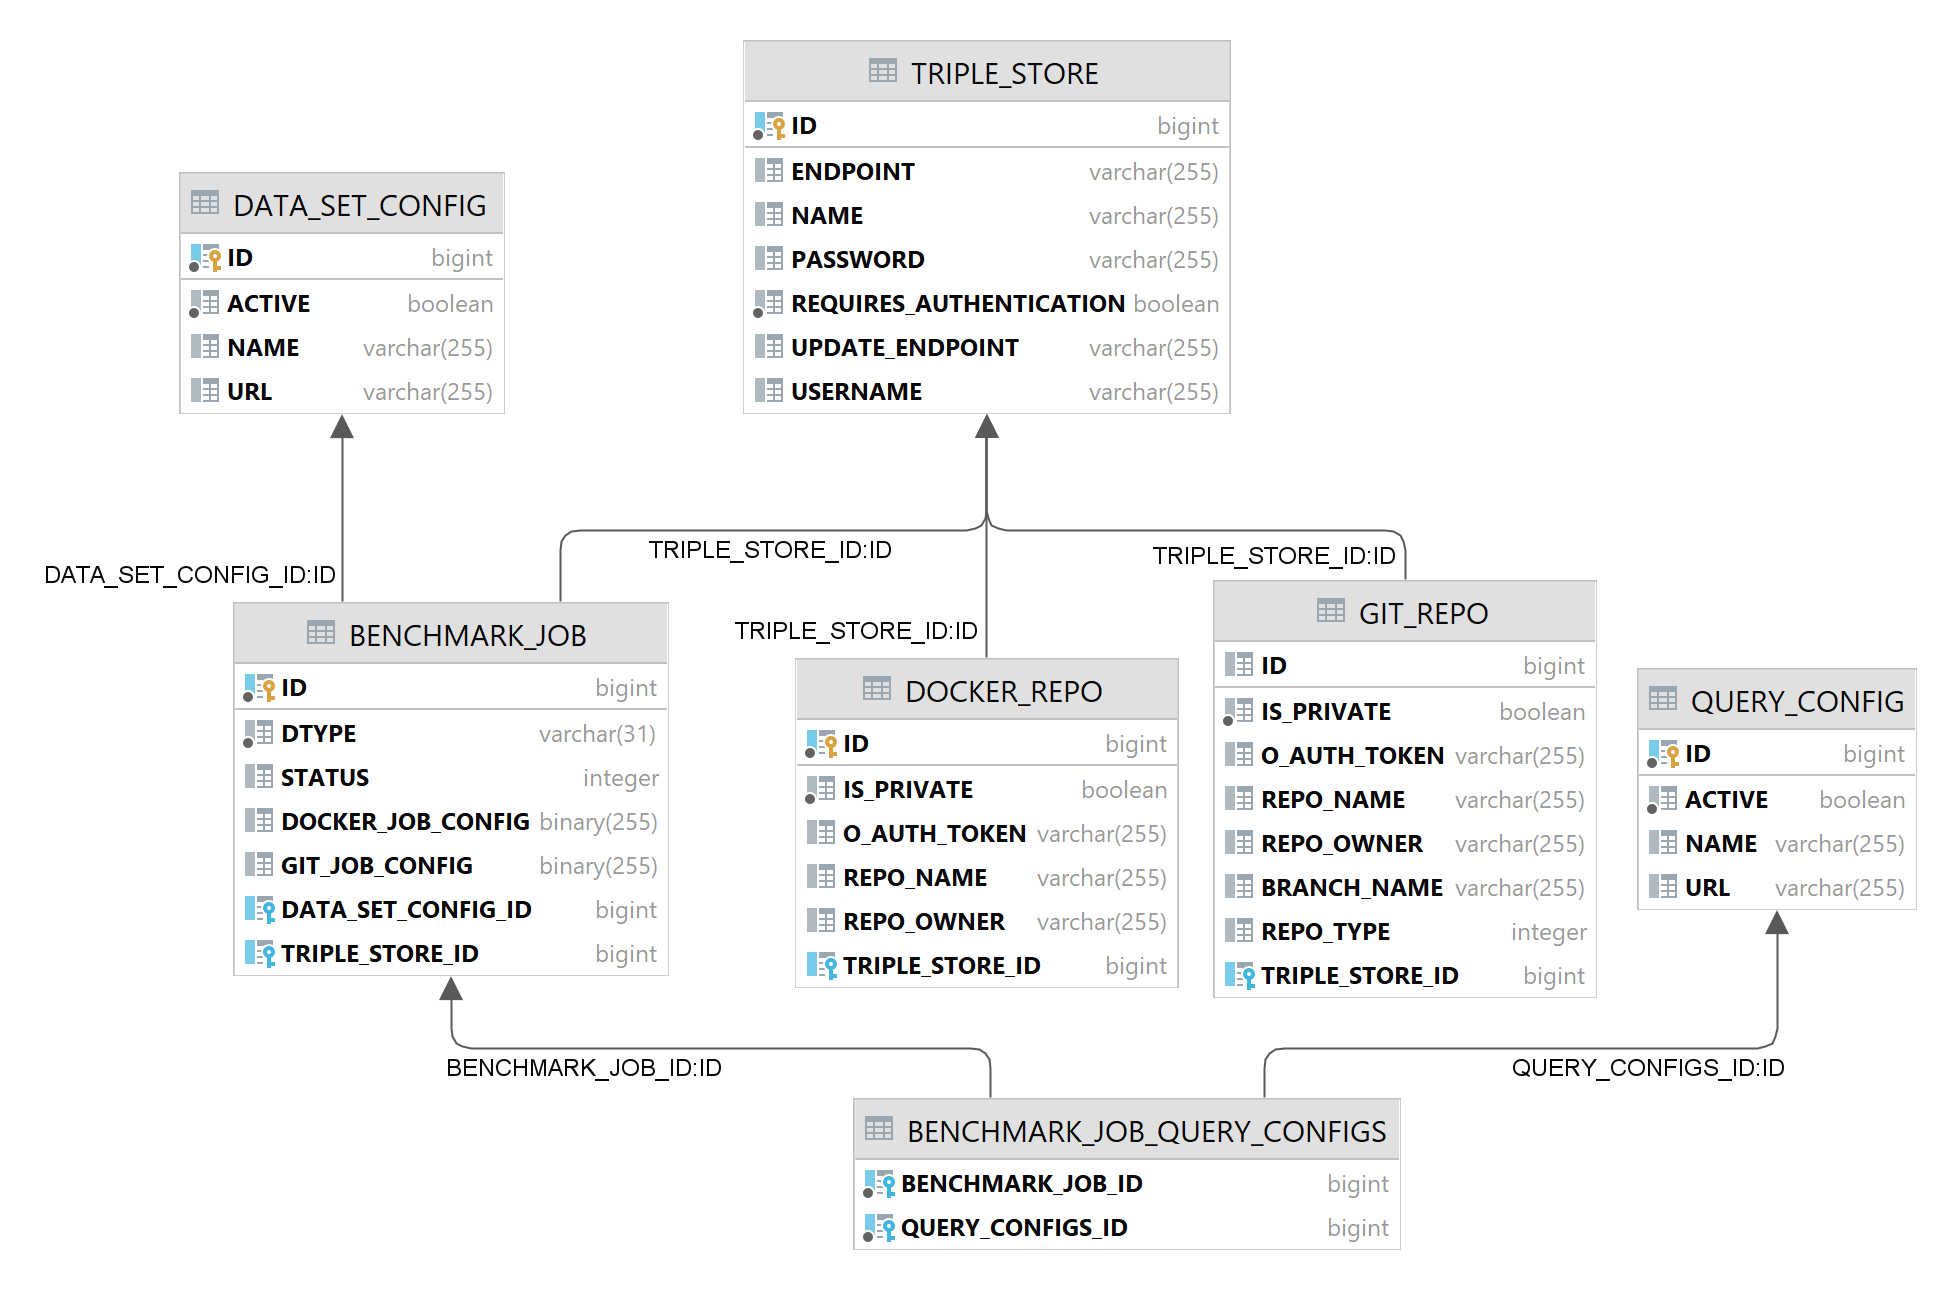
\includegraphics[width=.75\textwidth]{figures/jms_db_schema_design.png}
	\caption{Diagram of the proposed database schema for the \ac{jms}}
	\label{fig:design_jms_db_schema}
\end{figure}

This design takes advantage of persistence technology already part of the Spring framework.
The models for the \gh{} and \dockh{} are inherited from an abstract repository class since the basic information like repository name and owner are needed for both repository types.
The Spring framework automatically manages the different repositories and identifies them through the stored \texttt{DTYPE}.

Secondly, the relationship between \ac{ts} configurations and repositories is inverted. 
Now each repository points to a \ac{ts} configuration.
This means a \ac{ts} configuration can be used for different observed repository setups.

Lastly, the benchmark job and dataset models are cleaned up.
Now each benchmark specifies a dataset and a query file as well as multiple parameters, which are later used by \iguana{} during the execution of a benchmark job.
Each benchmark is now a single entry in the benchmark table.

The individual repositories and benchmarks are then linked inside a benchmark job.


\subsection{Creation and Management of Benchmark Jobs}
\label{sec:creation_of_benchmark_jobs_design}
Section \ref{sec:creation_of_benchmark_jobs} described how the creation of benchmark jobs needed to be changed in the \ac{jms}.
As explained in section \ref{sec:data_model_restructure_jms}, benchmarks are now stored in a database table and have a single dataset and query file.

When a new message about a new release arrives, the \ac{jms} will now create a benchmark job for each benchmark that is configured in Basilisk.
\\

To manage the created benchmark jobs, new API endpoints are created to get a list of all benchmark jobs and to abort jobs that have not yet been started.


\subsection{Hooks for Pull Requests in \gh{} Repositories}
\label{sec:pullrequests_hcs_design}
Currently, the Basilisk platform can not check for new pull requests published to an observed repository.
This functionality would greatly support the continuous benchmarking during the development process of \tsp{}.

As explained in chapter \ref{ch:approach}, \tsp{} are often developed by teams who collaboratively work on Git repositories.
A pull request is a standard way of introducing a newly developed feature to a source code repository.
Pull requests contain a description of the proposed changes, and the name of the development branch which should be pulled into the main branch of the repository.

Often these changes are developed in a forked repository.
A forked repository is an independent copy of the main repository.
\gh{} provides functionality to merge the latest changes of the original repo into the forked repo.
To send changes from the forked repo to the original repo, a pull request is needed.

In this forked repo, the developer can work independently on his changes and later create the pull request to the original repository.

The difficulty for the Basilisk platform is that these pull requests can stem from these forked repositories.
Since the repository containing the changes has a different URL than the original repo observed by the Basilisk platform, more information than usual is required to create and run a benchmark job for a pull request.
\\

The solution we designed for this issue is an extended message.
This message gets sent in the situation in which the pull requests originate from a different repository.
The message contains the URL, repository, and branch name for the \gh{} repository.
Therefore the message handling in the \ac{hcs} and \ac{jms} needs to be adjusted to handle this new message type.

The benchmark jobs and the \acl{tbs} did not need to be changed.
It is not relevant for a benchmark if the repository from which the Docker container is built differs from the observed repository.


\subsection{Missing Implementations in the \acl{jms}}
In this section we describe how the missing implementations are developed that are listed in section \ref{sec:review_missing_impl}.

The tasks for the \ac{hcs} are already dealt with in sections \ref{sec:management_repo_config_design} and \ref{sec:pullrequests_hcs_design}.
Also, the tasks for the \ac{jms} regarding the management and aborting of benchmark jobs are dealt with in section \ref{sec:creation_of_benchmark_jobs_design}.

Lastly, only the REST APIs for adding and removing the configurations of \tsp{} and benchmarks need to be added to the \ac{jms}.
Since the basic functionality of those endpoints is similar to the endpoints for adding and removing repositories, it is straightforward to implement those endpoints.
The configuration and relationships of the added data models are based on the data model designed in section \ref{sec:data_model_restructure_jms}.


%%%%%%%%%% Triplestore Benchmark Service
\subsection{\acl{tbs}}
The implementation of the \acl{tbs} was lacking significant parts of its functionality.
To explain the implementation steps, we follow the benchmarking process that is used when a new benchmark job is sent to the \ac{tbs}.
\\

The \ac{jms} sends the created benchmark jobs via the message queues of RabbitMQ.
The \ac{tbs} stores these jobs internally in a job queue.
Benchmark jobs can be manually aborted by the user over the REST API of the \ac{jms}.
When a benchmark job is aborted, the \ac{jms} will send a message to the \ac{tbs}.
If the job has not been processed yet, the \ac{tbs} will skip the job when looking for the next job to run.
\\

When a benchmark job is started, the \ac{tbs} needs to create a Docker image first that contains the \ts{} that will be benchmarked.
Afterward, a container is built and configured from the image.
The configuration is stored in the data model of the \ac{jms} and is provided with the benchmark job to the \ac{tbs}.
Then, the \iguana{} configuration file is created, and the framework gets started.
After \iguana{} performed the benchmark on the Container, \iguana{} writes the results to the \ac{jsts} and the \ac{tbs} stops and removes the Docker container.

The implementation of this process is explained in the following sections.


\subsubsection{Creation of Docker Images}
The setup and creation of the Docker images containing the \ts{} for a benchmarking job can be divided into two branches.
Triplestores from \dockh{} repositories are easier to setup than \tsp{} stored in \gh{} repositories.

For a benchmark of a \ts{} that is configured as a \dockh{} repository, the only task is to pull the Docker image from \dockh{} by providing the repository name and owner and the image tag that marks the new release.

The creation of a Docker image from a \gh{} repository is more complicated than simply downloading an image from \dockh{}.
First, the source code of the repository has to be downloaded. 
Then the Dockerfile needs to be located, and a build needs to be initiated, which often requires additional parameters and configurations.
Because of this increased complexity, we focused on the benchmark process of \dockh{} repositories.
As explained in the time schedule (\ref{sec:time_schedule}), the priority was to implement a fully running process, which was easier to accomplish for a \dockh{} repository.
\\

After creating of the Docker image, the benchmark process is the same for both repository types.


\subsubsection{Creating and Starting a Docker Container}
After the Docker image is available, a Docker container is configured and started.

The \ts{} which is the target of the benchmark job, will be run in the Docker container.
For a successful benchmark, the \ts{} needs to be accessible from the \ac{tbs} and also needs access to the dataset to calculate the results for the benchmark queries.

To be accessible from outside the container, the container is configured to expose and listen to specific ports on the network.
Through these ports, the SPARQL endpoint will be accessible, which \iguana{} uses to send queries and receive the results.

To give the \ts{} access to the dataset of the benchmark, the dataset can be provided in two different ways.
Either it is available inside the Docker container through a published volume provided by the server.
In this case, the \ts{} can use the file directly from the file system.
The second option is to provide the dataset by uploading it through the SPARQL endpoint of the running \ts{}.
For this option, a shell script needs to be provided by the \ts{} configuration.
This script is executed by the \iguana{} framework before the benchmark is started.

After these configurations, the container gets started, and the actual benchmark can run.


\subsubsection{Configuration and Start of the IGUANA Framework}
The actual benchmark is performed by the \iguana{} framework (\ref{sec:iguana}).
The framework takes a YAML or JSON file containing the benchmark configuration as the start parameter.
Therefore the \ac{tbs} creates this configuration file from the provided information of the current benchmark job.
This contains the name of the dataset, the address of the SPARQL endpoint, and the configuration of the benchmark to be performed.
The benchmark configuration contains the location of the query file and possible time limits or thread counts for the \iguana{}-workers.
Lastly, the connection for the \ac{jsts} is provided.
This connection is used after the benchmark to write the benchmark results to the storage.
The \iguana{} configuration gets encoded in JSON and is written to a temporary file on the server.
\\

The next step is to start the benchmark by starting the \iguana{} framework with the created benchmark configuration.
The \iguana{} framework is located on the server as an executable jar file.
It gets started as an individual process on the server with the configuration file as the argument.
If the dataset needs to be loaded after the \ts{} is started, \iguana{} executes the provided loading script first before starting the actual benchmark.


\subsubsection{REST Endpoint to Control Job Starting}
To have a better control of the execution of the benchmark jobs, the \ac{tbs} is extended with a REST endpoint that can start or stop the execution service.
This functionality works similarly to the \ac{hcs}.
When the service is started over the endpoint, the queue of benchmark jobs is read, and the next job in the queue is started.
When the user decides to stop the benchmark execution service, the running job will be finished, but no new job will be started from the job queue.


\subsubsection{Benchmark Cleanup}
When the \iguana{} framework has finished the benchmark, some cleanup is happening to free server resources.
This includes removing the \iguana{} configuration file, the Docker container, and the Docker image.
The Docker container gets stopped and removed by the \ac{tbs}.
After that, the Docker image is also removed to free up disk space.

